\documentclass[english,xcolor=svgnames]{beamer}

\input{../../../../Templates/Latex/teachingslidesbeamer.tex}


% ===========================================================
% ===========================================================
% ===========================================================
\begin{document}

\title{Evidence on Nominal Rigidities}
\vspace{1cm}
\author[shortname]{
\begin{tabular}{c}
	Johannes Wieland \\ 
	\footnotesize \href{mailto:jfwieland@ucsd.edu}{jfwieland@ucsd.edu}  \\ 
\end{tabular}
}

\date{Spring \the\year}

\setbeamertemplate{footline}{}
\makebeamertitle
\setbeamertemplate{footline}[frame number]{}

\addtocounter{framenumber}{-1}



%%%%%%%%%%%%%%%%%%%%%%%%%%%%%%%%%%%%%%%%%%%%%%%%%%
\AtBeginSection[]{
\setbeamertemplate{footline}{}
  \frame<beamer>{ 

    \frametitle{Outline}   

    \tableofcontents[currentsection] 
  }
\setbeamertemplate{footline}[frame number]{}
\addtocounter{framenumber}{-1}
}

\AtBeginSubsection[]{
\setbeamertemplate{footline}{}
  \frame<beamer>{ 

    \frametitle{Outline}   

    \tableofcontents[currentsection,currentsubsection] 
  }
  \setbeamertemplate{footline}[frame number]{}
  \addtocounter{framenumber}{-1}
}



%\setbeamertemplate{footline}{}
%\begin{frame}
%\frametitle{Outline}   
%\tableofcontents[hideallsubsections] 
%\end{frame}
%\addtocounter{framenumber}{-1}
%\setbeamertemplate{footline}[frame number]{}

%%%%%%%%%%%%%%%%%%%%%%%%%%%%%%%%%%%%%%%%%%%%%%%%%%
\section{Intro}
%%%%%%%%%%%%%%%%%%%%%%%%%%%%%%%%%%%%%%%%%%%%%%%%%%
\begin{frame}
\frametitle{Empirical Evidence on Role of Money}
\begin{itemize}
	\item  Big questions in monetary economics:
	\begin{itemize}
		\item How is an economy with money different from an economy without money?
		\item What effects do change in monetary policy have on real activity and inflation?
	\end{itemize}
	\item Our standard monetary model implied money was neutral. What is the empirical evidence?
	\begin{enumerate}
		\item Today: VARs
		\item Next class: Other approaches
	\end{enumerate}
\end{itemize}
\end{frame}


%%%%%%%%%%%%%%%%%%%%%%%%%%%%%%%%%%%%%%%%%%%%%%%%%%
\section{VARs}
%%%%%%%%%%%%%%%%%%%%%%%%%%%%%%%%%%%%%%%%%%%%%%%%%%

\begin{frame}
\frametitle{Introduction to VARs}
\begin{itemize}
\item Before we get started, introduce a key econometric tool: Vector Autoregression or VAR.	
	\begin{itemize}
	\item Proposed by Sims (1980), who won the Nobel Prize for it.
	\item Wanted a way to describe economic time series with minimal theoretical restrictions.
	\end{itemize}
	\item This is a key tool in macro to summarize relationships between macroeconomic time series.
	\begin{itemize}
	\item To motivate / test models.
	\item Examine response to structural shocks.
	\item Frequently used at central banks.
	\end{itemize}
\end{itemize}
\end{frame}


\begin{frame}
\frametitle{Stationarity and White Noise}
\begin{itemize}
	\item Cannot find regularities if things do not repeat themselves.
	\item Leads to concept of stationarity.
\begin{itemize}
	\item A time series $\{x_t\}$ is stationary if the mean, variance, and autocorrelation can be well approximated by sufficiently long time averages.
	\item $\{x_t\}$ is covariance stationary iff:
	\begin{align*}
		E{x_t}=\mu\;\forall\;t\text{ and }E\{(x_t-\mu)(x_{t-k}-\mu)\}=g_k\;\forall\;t,k
	\end{align*}
	\item Sometimes not a great assumption (e.g., economies in transition), but for post-war US GDP, it works.
	\item Otherwise, detrend or difference.
	\end{itemize}
	\item A \emph{white noise process} has mean zero, a constant variance, and is serially uncorrelated.
\end{itemize}
\end{frame}


\begin{frame}
\frametitle{Autoregressions}
\begin{itemize}
	\item An \emph{autoregression} is a regression of a time series $\{x_t\}$ on lags of itself.
	\item Example: AR(1)
	\begin{align*}
		x_t = \beta_0+\beta_1x_{t-1}+\epsilon_t
	\end{align*}
\begin{itemize}
	\item Stationary and stable if $|\beta_1|< 1$ and $\epsilon_t$ is white noise.
	\item Otherwise goes off to infinity and never mean reverts.
	\end{itemize}
	\item Can estimate $AR(N)$
	\begin{align*}
		x_t = \beta_0+\sum_{s=1}^{N}\beta_s x_{t-s}+\epsilon_t
	\end{align*}
	by OLS if $\{x_t\}$ is stationary.
\end{itemize}
\end{frame}


\begin{frame}
\frametitle{Vector Autoregression}
\begin{itemize}
	\item A vector autoregression is a generalization of an autoregression in which $x_t$ is a \emph{vector} of time series.
	\item Simple example we will use:
	\begin{align*}
		x_t = \left[\begin{matrix}y_t \\ z_t\end{matrix}\right]
	\end{align*}
	\begin{itemize}
		\item Can be of arbitrary size $n$.
	\end{itemize}
	\item The \emph{reduced-form} of a VAR(1) is then
	\begin{align*}
		x_t = A_0+A_1 x_{t-1}+e_t
	\end{align*}
	where $A_0$ is an $n\times1$ vector and $A_1$ is an $n\times n$ matrix.
\end{itemize}
\end{frame}

\begin{frame}
\frametitle{Reduced-Form VAR: Estimation}
\begin{itemize}
	\item More generally, for a VAR of size n with P lags,
	\begin{align*}
		x_t = A_0+\sum_{s=1}^P A_s x_{t-s}+e_t
	\end{align*}
	where $x_t,A_0,e_t$ are $n\times1$ vectors and $A_i$ are $n\times n$ matrices.
	\item There are thus $n + pn^2 $ coefficients and $(n + 1) n/2 $ in the variance-covariance matrix.
	\item The right hand side only contains predetermined variables of a stationary process, and the error terms are assumed to be serially uncorrelated with constant variance (can relax).
	\begin{itemize}
		\item So can estimate each equation by OLS.
		\item Application of seemingly unrelated regression.
	\end{itemize}
\end{itemize}
\end{frame}


\begin{frame}
\frametitle{Forecasting
}
\begin{itemize}
	\item Can forecast using VAR:
	\begin{align*}
		E_t x_{t+1} &= A_0+A_1x_t \\
		E_t x_{t+2} &= A_0+A_1x_{t+1} =  A_0+A_1[A_0+A_1x_t]
	\end{align*}
	\item Often-used diagnostic tool is the forecast error variance
decomposition (FEVD).
\begin{itemize}
	\item Tells us proportion of variance of moments in $\{y_t\}$ or $\{z_t\}$ due to $e_{1,t}$ and $e_{2,t}$.
	\item Like a partial $R^2$ of forecast error by forecast horizon.
\end{itemize}
\end{itemize}
\end{frame}


\begin{frame}
\frametitle{Impulse Response Functions
}
\begin{align*}
	IR(n)=A_1^n \left[\begin{matrix}1 \\ 0\end{matrix}\right]
\end{align*}
\begin{itemize}
	\item This is called an \emph{impulse response function} to $e_{1t}$ and is a convenient way to represent how shocks  $\{e_{t}\}$ affect $\{x_{t}\}$
\begin{itemize}
	\item Can plot graphically and create standard error bands.
\end{itemize}
	\item Intuitively, this is the difference between two processes $\{x_t\}$ that are made up of identical shocks $\{e_t\}$ except in period $t$, where an additional unit one shock is added to $e_{1t}$.
\end{itemize}
\end{frame}


\begin{frame}
\frametitle{Structural VARs
}
\begin{itemize}
	\item Unfortunately, reduced form VARs are restrictive.
\begin{enumerate}[1.]
	\item No simultaneous causality.
	\item Shocks have to be uncorrelated and white noise.
\end{enumerate}
	\item Generalize to a structural VAR.
	\item Tackle problem 1 first and allow for simultaneous causality:
	\begin{align*}
		y_t &= b_{10}-b_{12}z_t + \gamma_{11}y_{t-1}+\gamma_{12}z_{t-1}+\epsilon_{yt} \\
		z_t &= b_{20}-b_{21}y_t + \gamma_{21}y_{t-1}+\gamma_{22}z_{t-1}+\epsilon_{zt}
	\end{align*}
	 where $\epsilon_{yt}$ and $\epsilon_{zt}$ are independent white noise processes.
	\begin{itemize}
		\item Cannot directly estimate because $z_t$ is correlated with $\epsilon_{yt}$ and $y_t$ is correlated with $\epsilon_{zt}$, violating exclusion restriction.
		\item E.g., the current interest rate is a function of the current output gap, but the current output gap is also a function of the current interest rate.
	\end{itemize}
\end{itemize}
\end{frame}

\begin{frame}
\frametitle{Reduced-Form Representation
}
\begin{itemize}
	\item Write structural VAR as a matrix:
	\begin{align*}
	\begin{bmatrix} 
	1 & b_{12} \\ b_{21} & 1
	\end{bmatrix}
	\begin{bmatrix} 
	y_t \\ z_t
	\end{bmatrix} &=
	\begin{bmatrix} 
	b_{10} \\ b_{20}
	\end{bmatrix} + 
	\begin{bmatrix} 
	\gamma_{11} & \gamma_{12} \\ \gamma_{21} & \gamma_{22}
	\end{bmatrix}
	\begin{bmatrix} 
	y_{t-1} \\ z_{t-1}
	\end{bmatrix}+
	\begin{bmatrix} 
	\epsilon_{yt} \\ \epsilon_{zt}
	\end{bmatrix} \\
		Bx_t &= \Gamma_0 + \Gamma_1 x_{t-1}+\epsilon_{t}
	\end{align*}
	\item Premultiply by $B^-1$ to get reduced-form representation:
	\begin{align*} 
		x_t &= A_0 + A_1 x_{t-1}+e_{t}
	\end{align*}
	where $A_0=B^{-1}\Gamma_0$, $A_1=B^{-1}\Gamma_1$, and $e_{t}=B^{-1}\epsilon_{t}$
	\item Note reduced form errors $e_t$ are of form:
	\begin{align*}
		e_{1t}=\frac{\epsilon_{yt}-b_{12}\epsilon_{zt}}{1-b_{12}b_{21}}
	\end{align*}
	\begin{itemize}
		\item Stationary white noise, but correlated with one another.
		\item For IRs and FEVDs, want responses to $\epsilon_t$ not $e_t$.
	\end{itemize}
\end{itemize}
\end{frame}


\begin{frame}
\frametitle{The Identification Problem
}
\begin{itemize}
	\item \emph{Cannot invert from reduced form to structural VAR unless add restrictions.}
	\item Reduced form has 9 unknowns, six as plus 3 terms of var-covar matrix:
	\begin{align*}
		y_t &= a_{10} + a_{11}y_{t-1}+a_{12}z_{t-1}+e_{1t} \\
		z_t &= a_{20} + a_{21}y_{t-1}+a_{22}z_{t-1}+e_{2t}
	\end{align*}
	\item Structural form has 10 unknowns, 8 $b$'s and $\gamma$'s plus 2 terms of
var-covar matrix (uncorrelated shocks):
	\begin{align*}
		y_t &= b_{10}-b_{12}z_t + \gamma_{11}y_{t-1}+\gamma_{12}z_{t-1}+\epsilon_{yt} \\
		z_t &= b_{20}-b_{21}y_t + \gamma_{21}y_{t-1}+\gamma_{22}z_{t-1}+\epsilon_{zt}
	\end{align*}
	\item Fundamentally under-identified.
	\begin{itemize}
		\item Intuitively, $e$'s depend on both $\epsilon_{yt}$ and $\epsilon_{zt}$ so cannot invert from $e$'s to $\epsilon$'s. Extra parameters determine this relationship.
	\end{itemize}
\end{itemize}
\end{frame}


\begin{frame}
\frametitle{Recursive VARs and Identification
}
\begin{itemize}
	\item Solution is recursive system:
	\begin{itemize}
		\item Assume $y_t$ has contemporaneous effect on $z_t$, but $z_t$ has no
contemporaneous effect on $y_t$.
		\item Jargon: ``order'' $y_t$ first, in the sense that it is ``causally prior.''
		\item E.g., monetary policy affects output with a lag.
	\end{itemize}
	\item System is:
	\begin{align*}
		y_t &= b_{10} + \gamma_{11}y_{t-1}+\gamma_{12}z_{t-1}+\epsilon_{yt} \\
		z_t &= b_{20}-b_{21}y_t + \gamma_{21}y_{t-1}+\gamma_{22}z_{t-1}+\epsilon_{zt}
	\end{align*}
	so
	\begin{align*}
		e_{1t}=\epsilon_{yt}\text{ and }e_{2t}=\epsilon_{zt}-b_{21}\epsilon_{yt}
	\end{align*}
	\item Exactly identified because one parameter ($b_{12}$) is now a zero. 9 parameters in both structural VAR and reduced form.
	\item Intuition: Can now distinguish $\epsilon_{yt}$ and $\epsilon_{zt}$ shocks.
	\begin{itemize}
		\item Only $\epsilon_{yt}$ shocks affect contemporaneous values of $y_t$.
		\item $e_{1t}$ attributed completely to $\epsilon_{yt}$; can invert $e$'s to get $\epsilon$'s.
	\end{itemize}
\end{itemize}
\end{frame}


\begin{frame}
\frametitle{Cholesky Decomposition
}
\begin{itemize}
	\item Lower triangular assumption on the structural residuals is called a Cholesky decomposition.
	\begin{itemize}
		\item Most common identification scheme for VAR.
	\end{itemize}
	\item Generalize this to $n$ variable and $p$ lag VAR.
	\begin{itemize}
		\item $B$ is then an $n\times n$ matrix.
		\item Exact identification requires $(n^2-n)/2$ restrictions between
the regression residuals and structural innovations.
		\item Cholesky does this by setting exactly $(n^2-n)/2$ values of the
$B$ matrix to zero.
	\end{itemize}
\end{itemize}
\end{frame}

\begin{frame}
\frametitle{Error Correlation Version
}
\begin{itemize}
	\item Assume instead there is no simultaneous causality but
$e_t = C\epsilon_t$ where $\epsilon_t$ are the independent structural shocks and C is an $n\times n$ matrix:
	\begin{align*}
		x_t=A_0+A_1 x_{t-1}+C\epsilon_t
	\end{align*}
	\item Equivalent to structural VAR
	\begin{align*}
		C^{-1}x_t=C^{-1}A_0+C^{-1}A_1 x_{t-1}+\epsilon_t
	\end{align*}
	\begin{itemize}
		\item Same as before. Recursive VAR if $C^{-1}$ is lower triangular.
		\item Same problem --- cannot tell apart shocks.
		\item Now direct relationship between $e$'s and $\epsilon$'s instead of
relationship arising through simultaneous causality.
	\end{itemize}
	\item Alternate interpretation of Cholesky: Assume $\epsilon_{zt}$ affects both $y_t$ and $z_t$ but $\epsilon_{yt}$ has no contemporaneous effect on $z_t$.
\end{itemize}
\end{frame}


\begin{frame}
\frametitle{Cholesky Decomposition: Key Assumptions
}
\begin{itemize}
	\item Cholesky is a STRONG assumption.
	\begin{itemize}
		\item No reverse-causality.
		\item No omitted variables correlated with ``lower ordered'' variables
and ``higher ordered'' variables.
		\item Strong exclusion restriction.
	\end{itemize}
	\item ``Ordering'' sounds innocuous. It's not.
	\begin{itemize}
		\item $n!$ possible ordering.
	\end{itemize}
\end{itemize}
\end{frame}


\begin{frame}
\frametitle{Other SVAR Identification Schemes
}
\begin{itemize}
	\item VARs criticized for being too reduced form.
	\item Structural VAR (SVAR) approach uses economic theory rather than Cholesky decomposition invert reduced form VAR to structural VAR (that is, to recover structural innovations from reduced form residuals).
	\begin{itemize}
		\item Must impose $(n^2-n)/2$ restrictions.
	\end{itemize}
	\item Examples:
	\begin{itemize}
		\item Gali (1999) splits Solow residual into tech and non-tech shocks by assuming that only tech shocks affect long-run productivity.
		\item Sign restrictions (Uhlig).
		\item Assuming cross-sectional regression holds
(e.g., Beraja, Hurst, and Ospina, 2016).
	\end{itemize}
\end{itemize}
\end{frame}

%%%%%%%%%%%%%%%%%%%%%%%%%%%%%%%%%%%%%%%%%%%%%%%%%%
\section{VAR Evidence}
%%%%%%%%%%%%%%%%%%%%%%%%%%%%%%%%%%%%%%%%%%%%%%%%%%

\begin{frame}
\frametitle{VAR Evidence on Non-Neutrality
}
\begin{itemize}
	\item Apply VARs to study the effects of monetary shocks.
	\item Key challenge is endogeneity.
	\begin{itemize}
		\item Changes in monetary policy occur for good reasons.
		\item Error term $\epsilon_t$ correlated with outcome:
		\begin{align*}
			\Delta y_t = \alpha +\beta \Delta i_t + \epsilon_t
		\end{align*}
	\end{itemize}
	\item Start with simple VAR from Stock and Watson (2001).
	\begin{itemize}
		\item 3 variables: inflation, unemployment, and Federal Funds interest rate.
		\item Order $\pi_t, u_t, R_t$ in recursive VAR.
		\begin{itemize}
			\item $\pi_t$ affects $u_t$ and $R_t$ contemporaneously but not vice-versa.
			\item $u_t$ affects $R_t$ contemporaneously but not vice-versa.
		\end{itemize}
		\item See paper for data description (FEVD, Granger Causality tests).
	\end{itemize}
\end{itemize}
\end{frame}


\begin{frame}
%\frametitle{Stock-Watson IRFs
%}
\centering
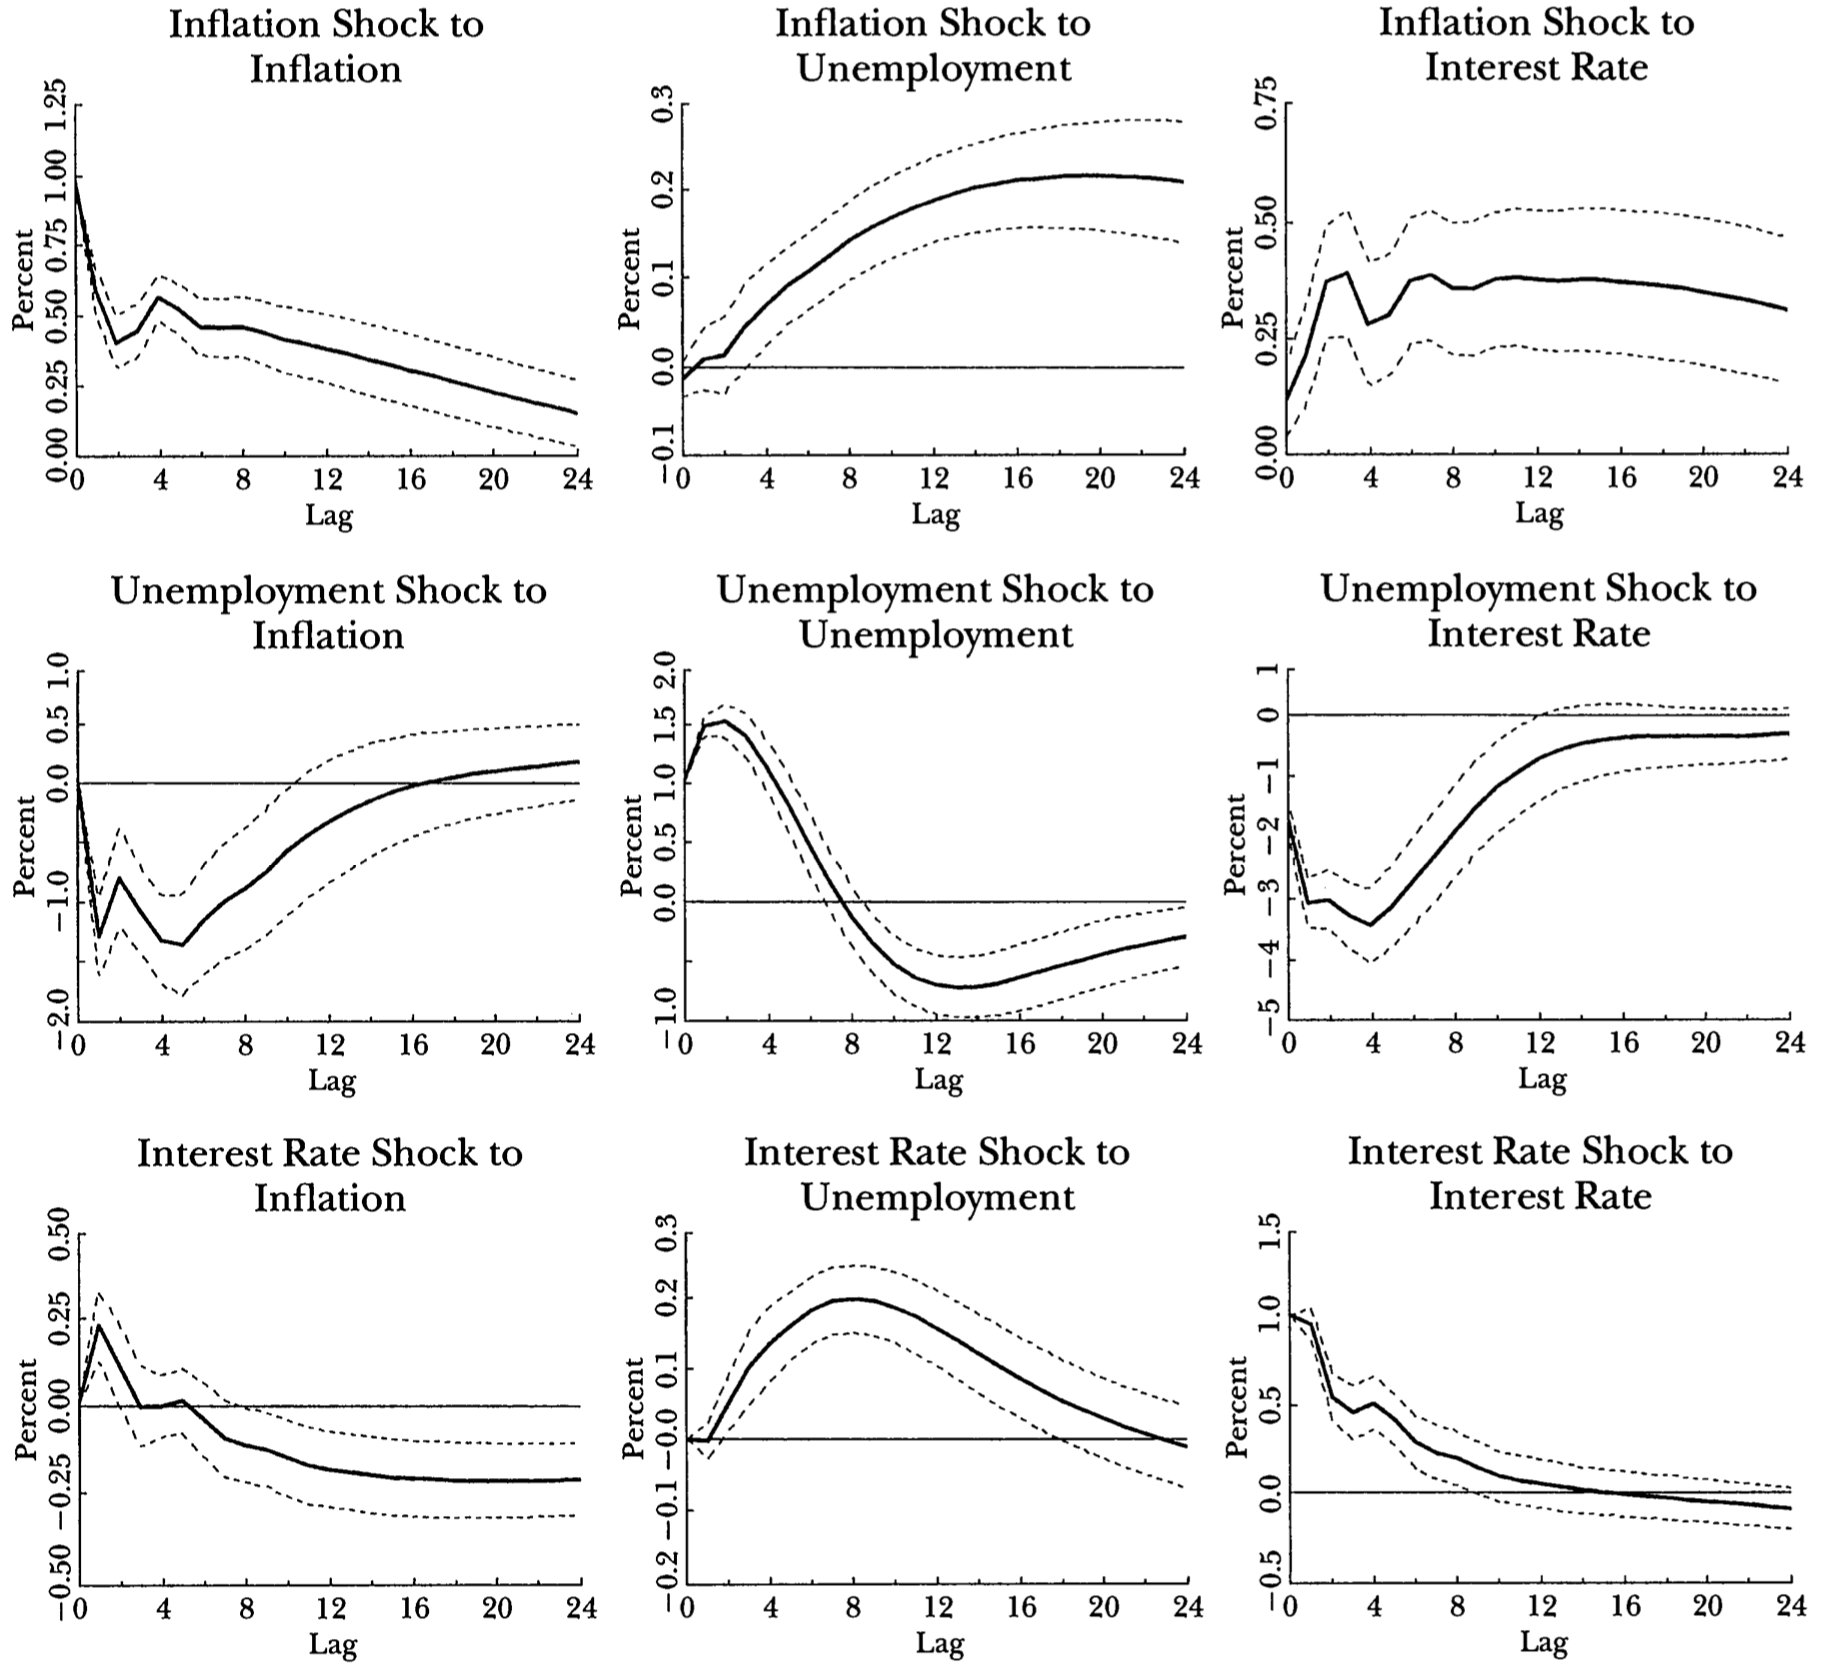
\includegraphics[scale=0.3]{../../Images/stockwatson2001irf.png}
\end{frame}


\begin{frame}
\frametitle{IRFs: Two Structural Approaches
}
\begin{itemize}
	\item Stock and Watson then use a structural VAR in which impose a Taylor rule for identification rather than recursive VAR.
	\begin{itemize}
		\item In solid: backward-looking Taylor rule.
		\item In dashed: forward-looking Taylor rule.
		\item Structural assumptions (and hence ordering) not innocuous.
	\end{itemize}
\end{itemize}
\centering
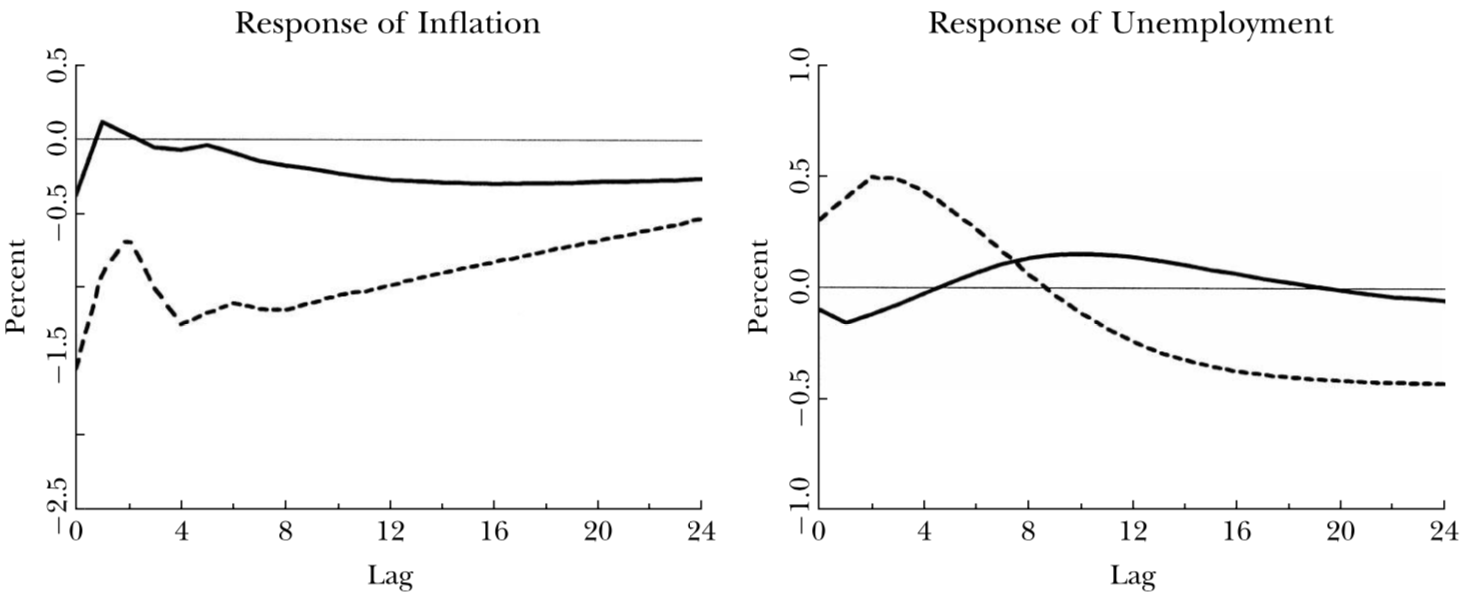
\includegraphics[scale=0.4]{../../Images/stockwatson2001structural.png}
\end{frame}

\begin{frame}
\frametitle{Christiano, Eichenbaum, and Evans (2005)}
\begin{itemize}
	\item Paper does a lot. For now just focus on VAR evidence.
	\item Run an 9-variable VAR. Ordering:
	\begin{enumerate}[1.]
		\item Real GDP
		\item Real Consumption
		\item GDP Deflator
		\item Real Investment
		\item Real Wage
		\item Labor Productivity
		\item Federal Funds Rate
		\item Real Profits
		\item M2 Growth
	\end{enumerate}
	\item Economic conditions can affect monetary policy, but monetary policy only affects economic conditions with a lag.
	\begin{itemize}
		\item Trying to get around endogeneity of monetary policy by statistically modeling it. But still Stock-Watson concerns.
	\end{itemize}
\end{itemize}
\end{frame}


\begin{frame}
\frametitle{CEE: IRF To Money Shock
}
\centering
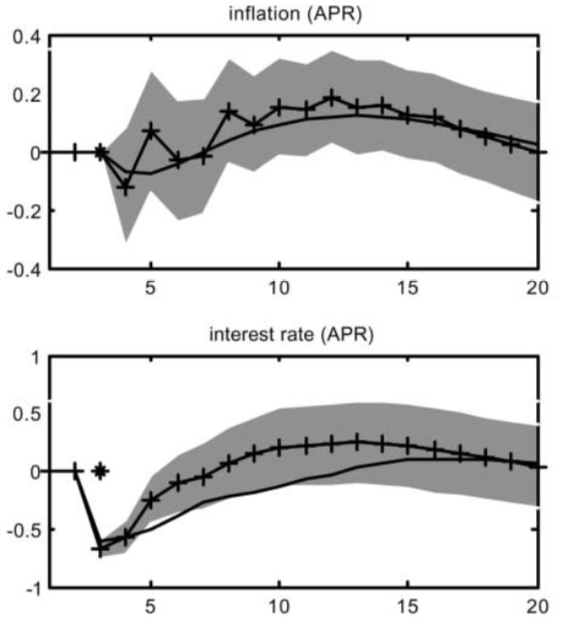
\includegraphics[scale=0.6]{../../Images/CEE2005-1.png}
\end{frame}

\begin{frame}
\frametitle{CEE: IRF To Money Shock
}
\centering
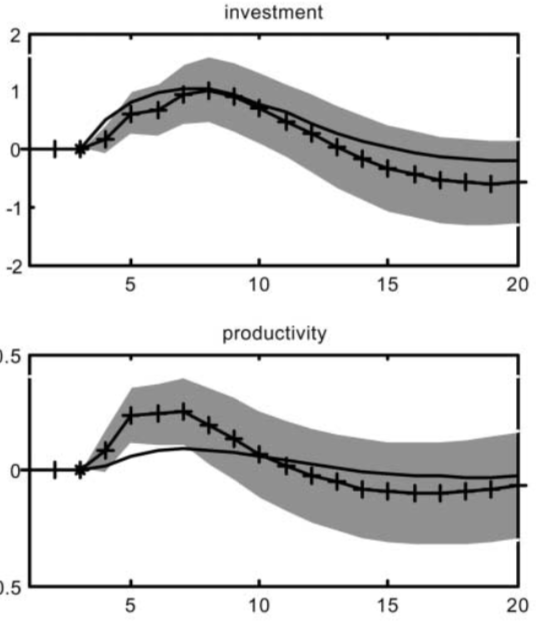
\includegraphics[scale=0.6]{../../Images/CEE2005-2.png}
\end{frame}

\begin{frame}
\frametitle{CEE: IRF To Money Shock
}
\centering
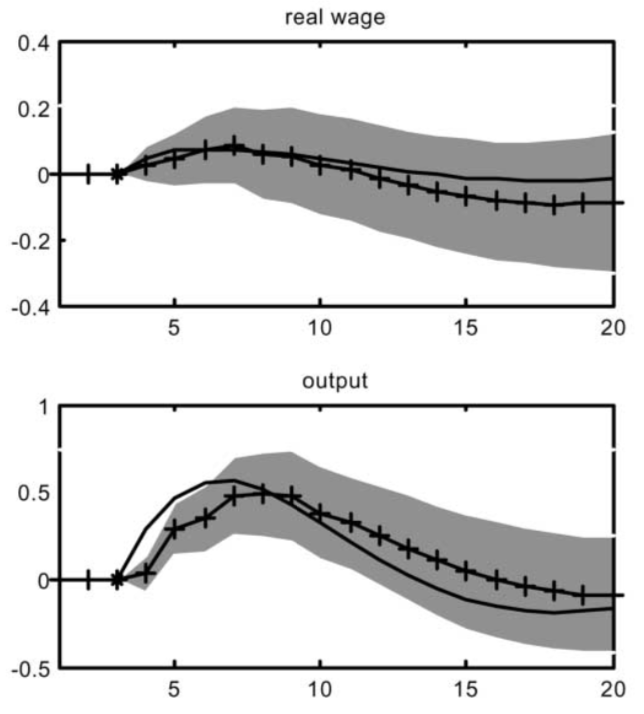
\includegraphics[scale=0.6]{../../Images/CEE2005-3.png}
\end{frame}

\begin{frame}
\frametitle{CEE: IRF To Money Shock
}
\centering
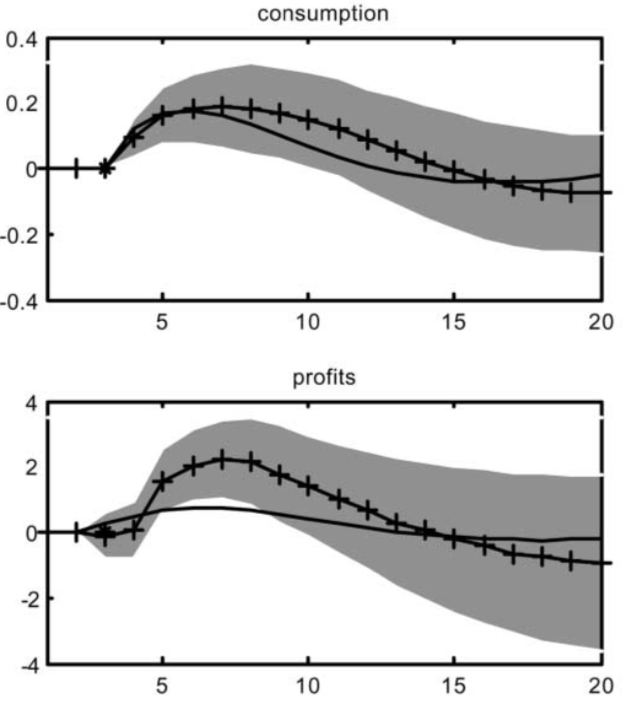
\includegraphics[scale=0.6]{../../Images/CEE2005-4.png}
\end{frame}

\begin{frame}
\frametitle{Christiano, Eichenbaum and Evans (2005) Summary}
\begin{enumerate}[1.]
	\item Hump-shaped response of output, consumption and investment, peaking at 1.5 years and returning to trend after 3.
	\item Hump-shaped response of inflation, peaking after two years.
	\item  Interest rate falls for one year
	\item Real profits, wages, and labor prod rise.
	\item Growth rate of money rises immediately.
\end{enumerate}
\begin{itemize}
		\item Phillips curve and Taylor rule as in Stock and Watson still hold.
		\item Consistent with significant \emph{monetary non-neutrality} $\Rightarrow$ money affects real outcomes.
	\end{itemize}
\end{frame}


%%%%%%%%%%%%%%%%%%%%%%%%%%%%%%%%%%%%%%%%%%%%%%%%%%
\section{Next Steps}
%%%%%%%%%%%%%%%%%%%%%%%%%%%%%%%%%%%%%%%%%%%%%%%%%%


\begin{frame}
\frametitle{Next Steps
}
\begin{itemize}
	\item VAR criticisms.
	\item Other approaches to identify real effects of money.
	\item Summary of the evidence.
\end{itemize}
\end{frame}


\end{document}